\section{ParaTwin: Digital Twin Design}\label{sec:twin}

Theorem~\ref{thm:hardness} establishes that the design space cannot be exhaustively optimized; the benchmarks (JD's deployed forecast--optimize--simulate loop \cite{wang2025}, Amazon's regionalization program \cite{chandra2026}) establish that the winning practice is a calibrated simulation--optimization loop. ParaTwin is that loop for ParagonCorp, in the sense of the digital supply chain twin literature \cite{ivanov2021,le2024,snoeck2022}.

\subsection{Formal Model}
\begin{definition}[ParaTwin]
ParaTwin is a discrete-event simulation \cite{law2015} defined by the tuple $\mathcal{T}=(\mathcal{X},\mathcal{E},\Phi,\Theta,\mathcal{Y})$: state $\mathcal{X}$ (inventory positions $I_{fk}(t)$, reservations $Q_{fk}(t)$, queue contents and picker occupancy, courier states, mid-mile shipments, open orders with promise clocks); events $\mathcal{E}$ (order arrival as marked spatial Poisson with campaign seasonality, basket sampler $\mathcal{B}_z$, live-commerce demand shocks as Hawkes bursts, routing decision, pick start/end, courier match/arrive/depart/deliver, replenishment wave dispatch/receipt, POS sale at store nodes, cycle-count adjustment, node outage, \emph{return and re-attempt}$^{\mathrm{R5}}$, \emph{connectivity loss and heartbeat gap}$^{\mathrm{R5}}$); dynamics $\Phi$; parameters $\Theta$; and the KPI vector $\mathcal{Y}$ of Table~\ref{tab:kpi} with confidence intervals from $\ge30$ independent replications under common random numbers \cite{law2015}.
\end{definition}

Crucially, routing transitions call the same ORE codebase as production and ATP transitions use the same VIS rules, so the twin and the network share decision logic by construction.

\subsubsection*{$^{\mathrm{R5}}$ The cost of sharing decision code}
Revision~4 presented shared decision code as an unqualified strength that eliminates model drift. It does eliminate drift, and it also removes independent verification of the decision logic. Trace-driven replay and holdout forecasting certify the \emph{environment} model against actuals; neither tests whether the routing cost model is correct, because the twin makes the same decision and then scores it. The exposure is concentrated in \emph{counterfactual} evaluation---candidate designs that were never run---which is exactly what the optimizer bank produces. A mis-scaled congestion shadow price in $c_{of}$ would bias every simulated design identically and pass certification.

Revision~5 adds an independent policy check: a fixed fraction of live waves is scored in shadow against a deliberately simple held-out policy (nearest-feasible node), and the realized difference is estimated off-policy \cite{li2011} and reported as a KPI. A decision model that cannot beat the naive policy on live traffic is not certified regardless of environment-model fit. This is validation of the decision, complementing Sargent's environment-validation framework \cite{sargent2013}.

\subsection{Scope and Calibration}
The twin is SKU-explicit, not aggregated: assortment decisions (Theorem~\ref{thm:assortment}), substitution, and bundle co-location effects are only visible at SKU granularity. Scale is tractable: 2,000 SKUs $\times$ ${\sim}150$ nodes is a $3\times10^5$-cell inventory state, small for a modern discrete-event engine. The item master and brand campaign calendars are synchronized nightly from MagPie/Heron masters; ParaTwin refuses to run a scenario whose master-data snapshot is stale ($>48$\,h), a governance rule that prevents the classic twin-drift failure.

Each production system publishes a calibration feed (Table~\ref{tab:contracts}). Validation is two-stage: \emph{trace-driven replay}---feed one historical week of real orders through the twin and require per-KPI deviation $\le10\%$ against actuals; then \emph{holdout forecasting}---simulate the next week ahead of time and score prediction intervals. A twin version is certified for decision use only after both gates pass, plus the independent policy check above; certification is re-run monthly.

\begin{table}[t]
\caption{ParaTwin Calibration Data Contracts. Feeds marked $^{\mathrm{R5}}$ are added in this revision.}
\label{tab:contracts}
\centering\footnotesize
\begin{tabular}{@{}p{1.5cm}p{4.4cm}p{1.4cm}@{}}
\toprule
\textbf{Source} & \textbf{Feed} & \textbf{Cadence}\\
\midrule
MagPie+ & Orders, baskets, promises, SLA outcomes; \emph{basket-size distribution $p_j$}$^{\mathrm{R5}}$ & streaming\\
Heron/Lite & Pick/pack event timestamps, accuracy, labour & streaming\\
Exagon+ & Store stock, POS postings, count variances; \emph{connectivity heartbeats}$^{\mathrm{R5}}$ & 5\,min\\
ShipGo+ & Courier quotes, ETAs, actual legs, mid-mile e-POD & streaming\\
Grab/GoSend & Zone-pair ETA/price distributions; \emph{joint availability}$^{\mathrm{R5}}$ & daily fit\\
MOSTRANS & Wave lead times, OTIF, temperature logs & per wave\\
Returns$^{\mathrm{R5}}$ & NDR, re-attempt, return-to-stock, QC failure & streaming\\
Market data & Campaign calendar, live-commerce schedule & weekly\\
\bottomrule
\end{tabular}
\end{table}

\subsection{Simulation--Optimization Loop}
Candidate designs are generated by the greedy and matroid algorithms of Section~\ref{sec:structural} (fast, with guarantees where the guarantees hold) and by the LP-rounding algorithms of \cite{chekuri2004,fleischer2011} where they do not, then evaluated in the twin under stochastic demand, courier variability and disruption scenarios; a ranking-and-selection procedure picks the certified winner \cite{snoeck2022,law2015}. The loop runs at three cadences: \emph{strategic} (quarterly: node openings, $n^\star$ re-estimation per Fig.~\ref{fig:cost}), \emph{tactical} (weekly: assortments $S_f$, base stocks $b_{fk}$, rosters $c_f$, wave length $\Delta$), and \emph{operational} (daily shadow mode: the twin replays yesterday against alternative routing policies and flags regret above threshold).

\begin{figure}[t]
\centering
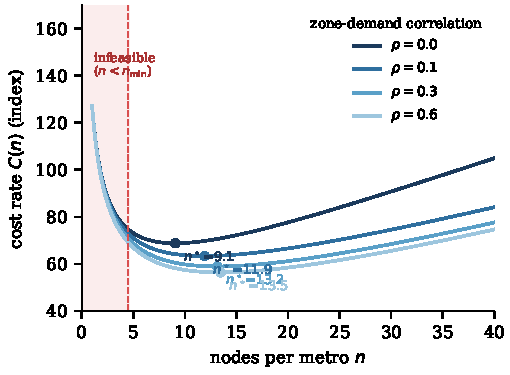
\includegraphics[width=\columnwidth]{costcurve.pdf}
\caption{$^{\mathrm{R5}}$ Illustrative ParaTwin design curve for one metro. Total cost \eqref{eq:cost} is unimodal in $n$; the minimizer $n^\star$ moves right as zone-demand correlation $\rho$ rises, because correlated demand cannot be pooled and decentralization therefore costs less. Revision~4 reported only the $\rho=0$ curve. The network is sized at $\max(n_{\min},n^\star)$, with $n_{\min}$ from Proposition~\ref{prop:radius}; the shaded band marks the SLA-infeasible region. Parameters $(F,a,b)=(1.2,6,120)$ are illustrative and are not Jakarta values.}
\label{fig:cost}
\end{figure}

\subsection{Experiment Portfolio and KPIs}
The launch experiment portfolio is: \textbf{E1} Jakarta node-count sweep $n\in\{5,\dots,40\}$ mixing store nodes and dark MFCs, reporting the curve of Fig.~\ref{fig:cost}; \textbf{E2} assortment depth ladder (150/300/600/1,200 SKUs) against PX1 capture, split-shipment rate, \emph{and order fill rate}$^{\mathrm{R5}}$; \textbf{E3} courier strategy (Grab-only versus dual-carrier versus own-fleet threshold search); \textbf{E4} campaign stress ($10\times$ Hawkes burst during a live event; measures promise-degradation behaviour); \textbf{E5} disruption (hub outage, flood-day travel times $+80\%$, courier surge) with \emph{jointly modelled carrier availability}$^{\mathrm{R5}}$; \textbf{E6} POS-latency and connectivity-outage sensitivity validating conditions (C1)--(C2) of Proposition~\ref{prop:atp}.

$^{\mathrm{R5}}$ Two experiments are added, and they are the only two that can falsify the program rather than tune it:

\textbf{E7 (demand test).} A live promise A/B on brand.com and one marketplace cluster, measuring instant attach rate, conversion lift versus the standard promise, and delivery-fee elasticity, for beauty baskets in Jakarta. E7 does not require the network: it requires a promise and a small number of nodes, and it runs in Phase~0. Revision~4 contained six supply-side experiments and no demand test, so the assumption on which every node economic rests---that Indonesian beauty consumers convert on a 60-minute promise at a rate that clears the break-even volume derived under O-17---was never scheduled to be measured.

\textbf{E8 (incrementality holdout).} A matched-market design over participating versus non-participating consignment stores of similar archetype and catchment, estimating the incremental share of store-node volume against the counterfactual of the walk-in sale \cite{imbens2015,abadie2010}. E8 resolves the contradiction between the partner-benefit and cannibalization framings of Section~\ref{sec:business}.

\begin{table}[t]
\caption{ParaTwin KPI Vector $\mathcal{Y}$ (per scenario, with 95\% CIs). Rows marked $^{\mathrm{R5}}$ are added in this revision.}
\label{tab:kpi}
\centering\footnotesize
\begin{tabular}{@{}p{1.3cm}p{6.3cm}@{}}
\toprule
\textbf{Group} & \textbf{KPIs}\\
\midrule
Promise & $\alpha$-attainment per class; p50/p95 click-to-door; promise-shown rate (\% of zone-hours with PX1 offered); \emph{promise-downgrade rate by cause}$^{\mathrm{R5}}$\\
Economics & Contribution/order (pick, courier, mid-mile, \emph{returns, packaging, commission}$^{\mathrm{R5}}$); routed mid-mile km and batching savings; node break-even attainment; network cost $C(n)$; \emph{incrementality ratio (E8)}$^{\mathrm{R5}}$\\
Inventory & \emph{Order fill rate $\alpha_B$}$^{\mathrm{R5}}$; item fill rate $\beta$; safety stock (units, IDR); substitution and split-shipment rates; expiry/obsolescence risk\\
Operations & Picker utilization; queue-delay probability vs.\ \eqref{eq:staffing}; courier match time; cycle-count variance; \emph{ORE regret vs.\ clairvoyant}$^{\mathrm{R5}}$; \emph{ORE lift vs.\ naive policy (off-policy)}$^{\mathrm{R5}}$\\
Resilience & SLA retention under E5 disruptions; recovery time; re-routing coverage; \emph{Boole-bound vs.\ fitted-quantile radius gap}$^{\mathrm{R5}}$\\
Demand$^{\mathrm{R5}}$ & Instant attach rate; conversion lift vs.\ standard promise; delivery-fee elasticity (E7)\\
\bottomrule
\end{tabular}
\end{table}
